%%%%%%%%%%%%%%%%%%%%%%%%%%%%%%%%%%%%%%%%%
% a0poster Portrait Poster
% LaTeX Template
% Version 1.0 (22/06/13)
%
% The a0poster class was created by:
% Gerlinde Kettl and Matthias Weiser (tex@kettl.de)
% 
% This template has been downloaded from:
% http://www.LaTeXTemplates.com
%
% License:
% CC BY-NC-SA 3.0 (http://creativecommons.org/licenses/by-nc-sa/3.0/)
%
%%%%%%%%%%%%%%%%%%%%%%%%%%%%%%%%%%%%%%%%%

%----------------------------------------------------------------------------------------
%	PACKAGES AND OTHER DOCUMENT CONFIGURATIONS
%----------------------------------------------------------------------------------------

\documentclass[a0,portrait]{a0poster}

% Custom packages/commands
\newcommand{\pff}{\texttt{pyforfluids }}
\newcommand{\conc}{\overline{x}}
\usepackage[svgnames]{xcolor} % Specify colors by their 'svgnames', for a full list of all colors available see here: http://www.latextemplates.com/svgnames-colors
\usepackage[edges]{forest}
\usepackage{fancybox}
\definecolor{background}{gray}{0.95}
\newcommand{\titleframe}[1]{
	\begin{frame} \null\hfill\huge{\shadowbox{#1}}\hspace{1cm} \end{frame}
}

\newcommand{\boxedeq}[2]{
	\begin{empheq}[box={\fboxsep=6pt\fbox}]{align}\label{#1}#2\end{empheq}
}

\newcommand{\coloredeq}[2]{
	\begin{empheq}[box=\colorbox{lightgreen}]{align}\label{#1}#2\end{empheq}
}

\newcommand{\fig}[3]{
	\begin{columns}
	\column{0.4\textwidth}
	\begin{figure}[htp] 
		\includegraphics[height=0.5\textheight,width=0.9\textwidth,
	keepaspectratio]{#1}\caption{#2}\end{figure}
	\column{0.6\textwidth}#3
	\end{columns}
}
\newcommand{\tabitem}{~~\llap{\textbullet}~~}

\newcommand{\htree}[1]{
	\begin{forest}
	for tree={
	fit=band,
	grow'=0,
	parent anchor=children,
	child anchor=parent,
	anchor=parent,
	if n children=0{folder}{},
	edge path'={(!u.parent anchor) -- ++(5pt,0) |- (.child anchor)},
	},
	where n=1{
	calign with current edge
	}{},
	#1
	\end{forest}
}

\usepackage[backend=biber,
	    style=authoryear-icomp,
]{biblatex}
\AtBeginBibliography{\tiny}
\addbibresource{sample.bib}

\usepackage{minted}
\setminted[python]{
    breaklines, framesep=2mm,
    fontsize=\footnotesize, numbersep=5pt, bgcolor=background,
}
% --------------

\usepackage{multicol} % This is so we can have multiple columns of text side-by-side
\columnsep=100pt % This is the amount of white space between the columns in the poster
\columnseprule=3pt % This is the thickness of the black line between the columns in the poster

\usepackage{graphicx} % Required for including images
\graphicspath{{figures/}} % Location of the graphics files
\usepackage{booktabs} % Top and bottom rules for table
\usepackage[font=small,labelfont=bf]{caption} % Required for specifying captions to tables and figures
\usepackage{amsfonts, amsmath, amsthm, amssymb} % For math fonts, symbols and environments
\usepackage{wrapfig} % Allows wrapping text around tables and figures

\begin{document}

%----------------------------------------------------------------------------------------
%	POSTER HEADER 
%----------------------------------------------------------------------------------------

% The header is divided into two boxes:
% The first is 75% wide and houses the title, subtitle, names, university/organization and contact information
% The second is 25% wide and houses a logo for your university/organization or a photo of you
% The widths of these boxes can be easily edited to accommodate your content as you see fit


\begin{tabular}{lr}
\begin{minipage}[b]{0.75\linewidth}
\huge \color{NavyBlue}
\textbf{PyForFluids: A Python package for multicomponent fluid
thermodynamic properties and phase equilibrium calculations.}
\color{Black}\\ % Title
\large \textbf{
Benelli, Federico E.$^1$; Arpajou, M. Candelaria $^2$; Cabral, Juan B. $^3$;
Cismondi, Martín $^1$
}\\[0.5cm] % Author(s)
\small 
$^1$ Instituto de Investigación y Desarrollo en Ingeniería de Procesos y Química Aplicada (IPQA-UNC-CONICET) \\
$^2$ INGAR Instituto de Desarrollo y Diseño (CONICET-UTN) \\
$^3$ Instituto de Astronomía Teórica y Experimental (IATE-OAC-CONICET)
\\[0.4cm] % University/organization
\Large \texttt{federico.benelli@mi.unc.edu.ar} \\
\end{minipage} & \hspace{3cm}
\begin{minipage}[b]{0.25\linewidth}
\vspace{-10cm}
\begin{center}
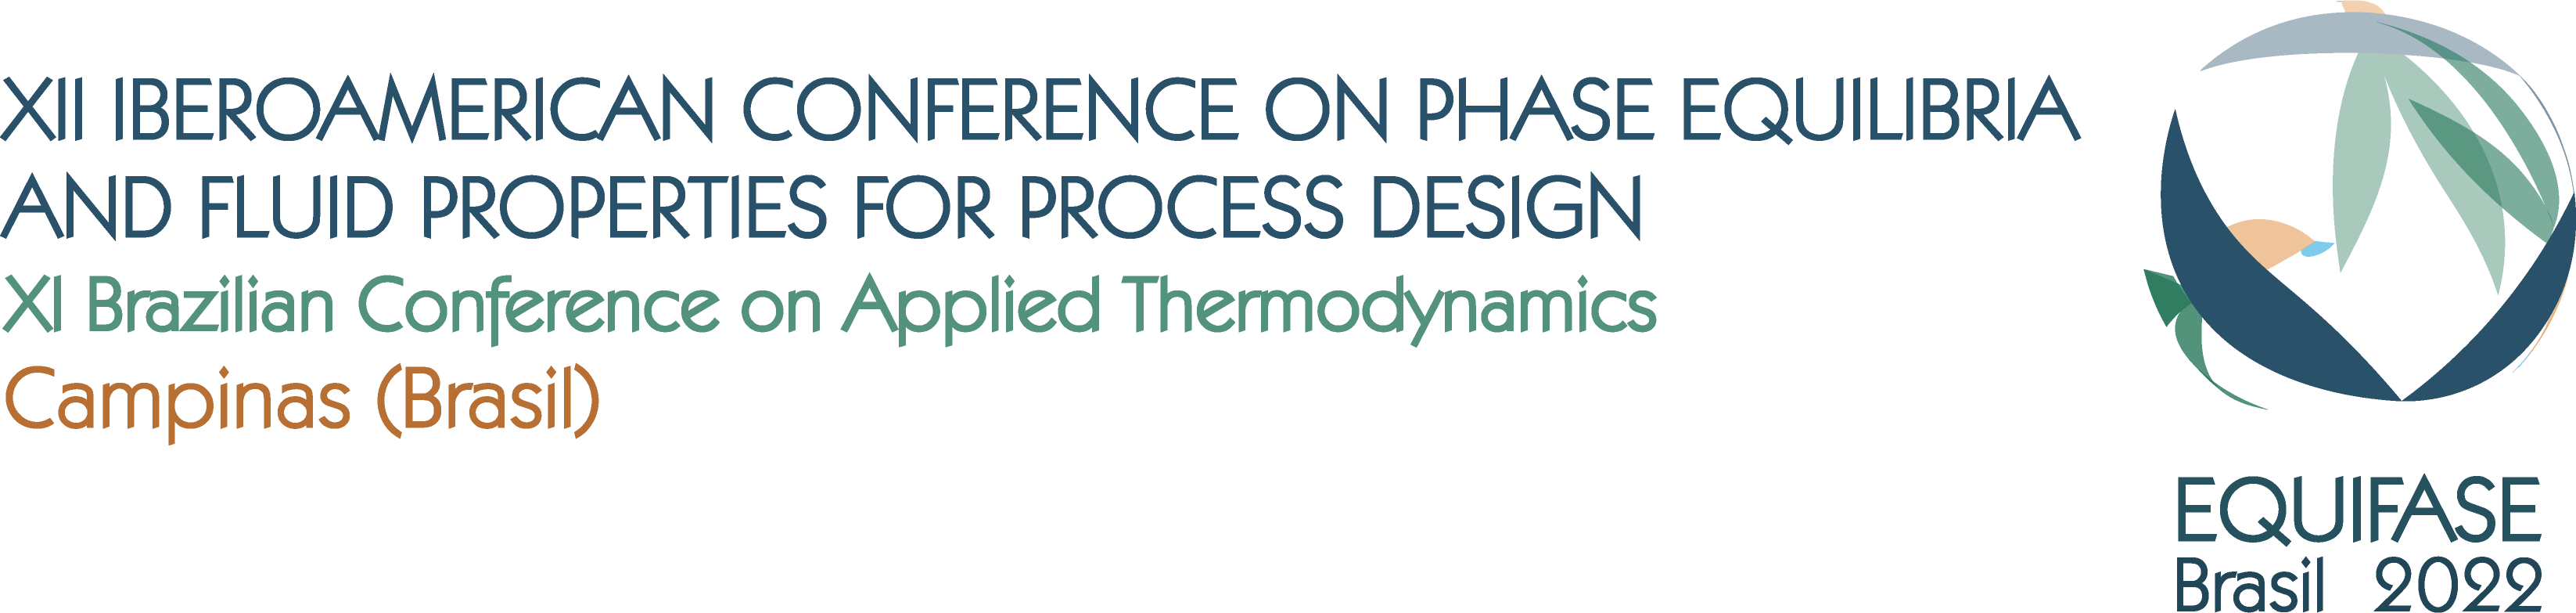
\includegraphics[width=15cm]{equifase-logo.png}

\includegraphics[width=10cm]{ipqa.png}\vspace{1cm}

\includegraphics[width=10cm]{ingar.png}

\includegraphics[width=10cm]{iate.png}
\\
\end{center}
\end{minipage}
\end{tabular}

\hrule

\vspace{1cm} % A bit of extra whitespace between the header and poster content

%----------------------------------------------------------------------------------------
\color{Navy} % Navy color for the abstract

\begin{abstract}

PyForFluids (Python-Fortran-Fluids) is a Python package focused on the
calculation of multicomponent fluids properties and phase equilibrium based on
Equations of State (EoS). It provides a simple interface to work from  a high
level object oriented abstraction but also exploits the high performance
Fortran code for the heavier calculations. Right now it includes the
multicomponent GERG-2008 EoS and three cubic EoS (Peng-Robinson,
Soave-Redlich-Kwong and RKPR) are being implemented. All four equations are
explicit in the Helmholtz Free Energy. PyForFluids calculates multiple
thermodynamic properties like speed of sound, isobaric heat, compressibility
factor, entropy, enthalpy, etc. Besides that, biphasic equilibrium calculations
like flash, bubble and dew points are included, with phase envelopes tracing
being in current development. To realize complex calculations, PyForFluids
takes advantage of the high performance and speed of Fortran code. At the same
time, it offers a user-friendly Python interface. The integration between these
two programming languages is achieved thanks to numpy module f2py. Fortran was
the chosen language due to both being faster for numerical routines  and an
availability of legacy projects. This package is designed with a collaborative
and modular approach in mind, taking advantage of an object oriented
programming approach. To both see the inner workings of it and make
changes/additions proposals all the code is available on an public repository
at GitHub https://github.com/fedebenelli/pyforfluids PyForFluids is made
following programming good practices standards for continuous integration. At
each code addition or modification, the package is tested with specific unit
tests to assure the reliance of the computations. Also the documentation where
each class and function is described is automatically generated and hosted at
pyforfluids.readthedocs.io with each update, where also a simple tutorial with
the basic usage of the package can be found.
\end{abstract}

\hrule

\begin{multicols}{2} % This is how many columns your poster will be broken
                     % into, a portrait poster is generally split into 2 columns

%----------------------------------------------------------------------------------------
%	ABSTRACT
%----------------------------------------------------------------------------------------


%----------------------------------------------------------------------------------------
%	INTRODUCTION
%----------------------------------------------------------------------------------------

\color{SaddleBrown} % SaddleBrown color for the introduction

\section*{Introduction}
\pff aim's to be a tool that provides robust fluid thermodynamic properties and
phase equilibria calculations, with focus in both simplicity in use and
extensibility, with the help of abstractions obtained with an object oriented
approach.


\color{DarkSlateGray} % DarkSlateGray color for the rest of the content

\subsection*{Implemented models}

\subsubsection*{GERG-2008}
The GERG-2008 EoS is a multicomponent equation of state, developed to be
implemented in natural gas usage, but it keeps a high accuracy for the whole
range from liquid to super critical conditions.\\

\textbf{Ideal term}

\begin{equation}
    \label{eq:ideal_term}
    \alpha^o (\conc, \rho, T) = \sum_{i=1}^{N} x_i\left[
    \alpha_i^o(\rho, T) + \ln x_i
    \right] 
\end{equation}

\textbf{Residual term}

\begin{equation}
    \label{eq:residual_term}
    \alpha^r(\conc, \delta, \tau) = 
    \sum_{i=1}^N x_i \alpha_i^r(\delta, \tau) +
    \sum_{i=1}^{N-1}\sum_{j=i+1}^N x_i x_j F_{ij}\alpha_{ij}^r(\delta, \tau)
\end{equation}

\begin{equation}
    \label{eq:residual_pure}
    \alpha^r_i(\delta, \tau) = \sum_{k=1}^{K_{Pol,i}} n_{i,k}\delta^d_{i,k} \tau^{t_{i,k}} +
    \sum_{k=K_{Pol,i}+1}^{K_{Pol,i}+K_{Exp,i}} n_{i,k} \delta^d_{i,k}\tau^{t_{i,k}}e^{-\delta^{c_{i,k}}}
\end{equation}

\subsubsection*{Cubic Equations of State}
\textbf{Residual term} 

\begin{equation}
    \alpha^r(T, V, n) = -n \ln(1 - B/V) - \frac{D(T)}{RTB(\delta_1 - \delta_2)}\ln\left(\frac{1+\delta_1 B/V}{1+\delta_2 B/V}\right)
\end{equation}

\subsubsection*{Available properties}
The available properties to calculate are dependant on the model being used.
Some of them are: $C_v$, $C_p$, $w$, $S$, $G$, $H$, $\mu_{JT}$, Virial Terms

\section*{Code Implementation}

\pff implementation is focused on two kind of Python objects:

\begin{description}
    \item[Fluid] A Fluid object that contains all generic procedures and
	attributes that can describe a Fluid.
    \item[Model] A Model object that contains all the relevant procedures
	related to an Equation of State. On \pff there are included two model
	objects \texttt{GERG2008} and \texttt{CubicEOS}.
\end{description}

These objects give the user the building blocks to implement 

\subsection*{Model Object}
A \texttt{Model} object contains all the necessary procedures to make
thermodynamic properties calculations and relevant constants required by
other functions (like $P_c$).\\

\htree{
[Model,
    [Constants, [\text{$R$, $T_c$ ,$P_c$, $\omega$}]]
    [Procedures, [
        [Components validator]
        [Concentration normalizer]
        [Properties calculator]
        ]
    ]
]
}

All these attributes and procedures are a \textbf{must have} for every model
since they are used by other external functions.

\begin{multicols}{2}

\emph{Defining a GERG2008 model}
\begin{minted}{python}
    import pyforfluids as pff

    gerg_model = pff.models.GERG2008()
\end{minted}
\vfill\null
\columnbreak

\emph{Defining a Peng Robinson model}
\begin{minted}{python}
    pr_model = pff.models.CubicEOS(
            model="PR",
            mix_rule="ClassicVdW",
            names=names,
            critical_temperature=tc,
            critical_pressure=pc,
            acentric_factor=w,
            kij_matrix=kij,
            lij_matrix=lij
    )
\end{minted}
\end{multicols}

\vspace{5cm}

\subsection*{Fluid Object}
A \texttt{Fluid} object contains the higher level procedures that are generic
for any kind of model.

\htree{
[Fluid,
    [Model]
    [State, [\text{composition, $P$, $T$, $\rho$}]]
    [Density solver]
    [Isotherms calculator]
    [Properties calculation \text{$f(N, T, \rho)$}]
]
}

\begin{multicols}{2}
\begin{minted}{python}
import pyforfluids as pff
import numpy as np

fluid = pff.Fluid(
    model=pff.models.GERG2008()
    composition={"methane": 0.2,
                 "ethane":  0.8},
    temperature=270 # K
    density=0.02 # mol/dm3
)
density_range = np.linspace(0.001, 20, 100)
isotherm = fluid.isotherm(density_range=density_range)
\end{minted}

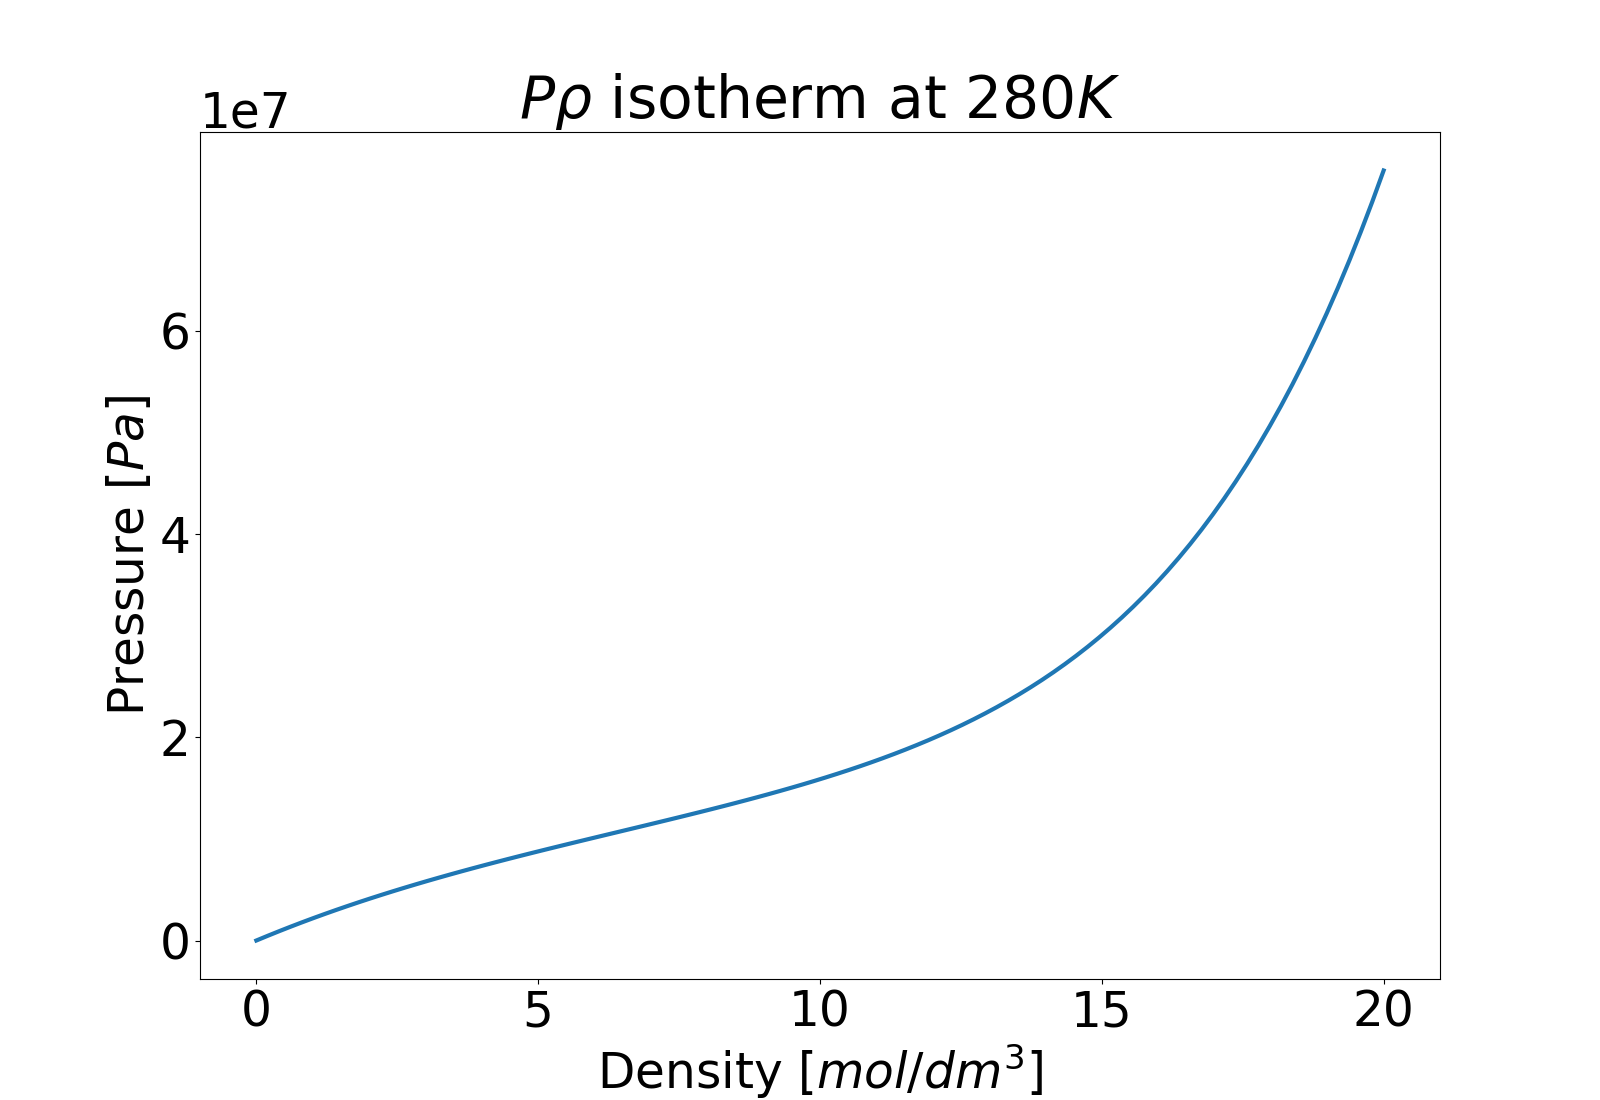
\includegraphics[width=17cm]{isotherm.png}
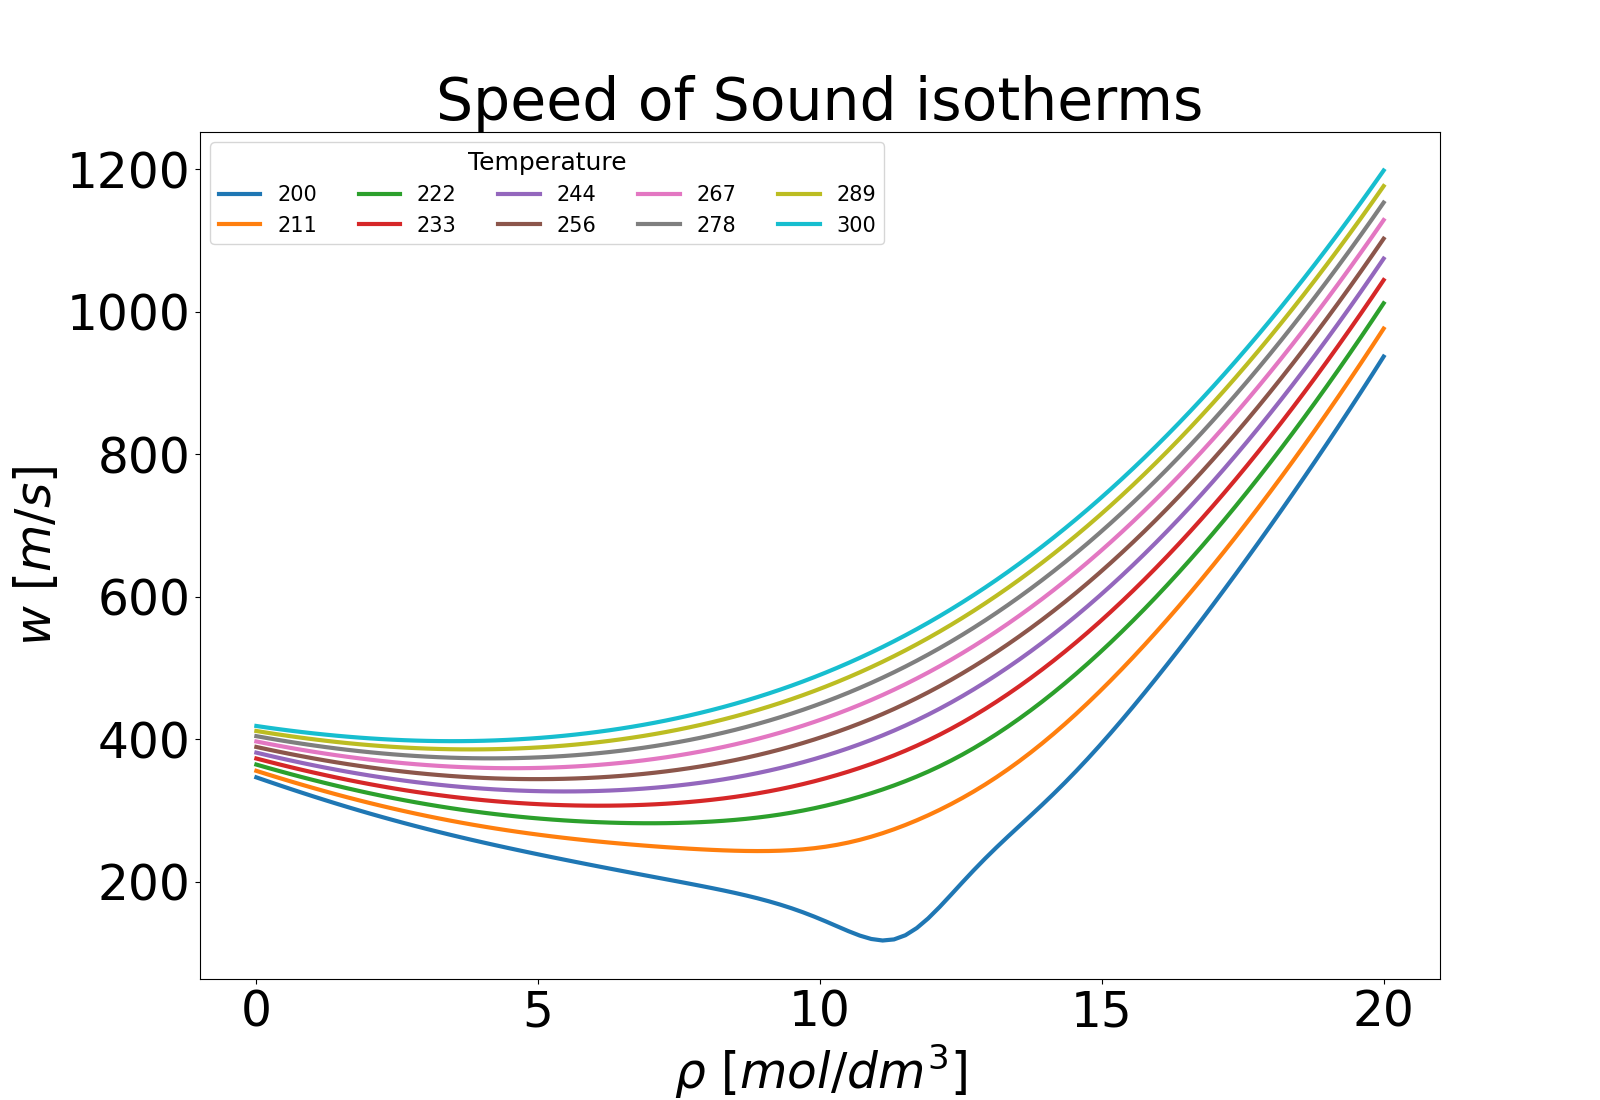
\includegraphics[width=17cm]{ss.png}
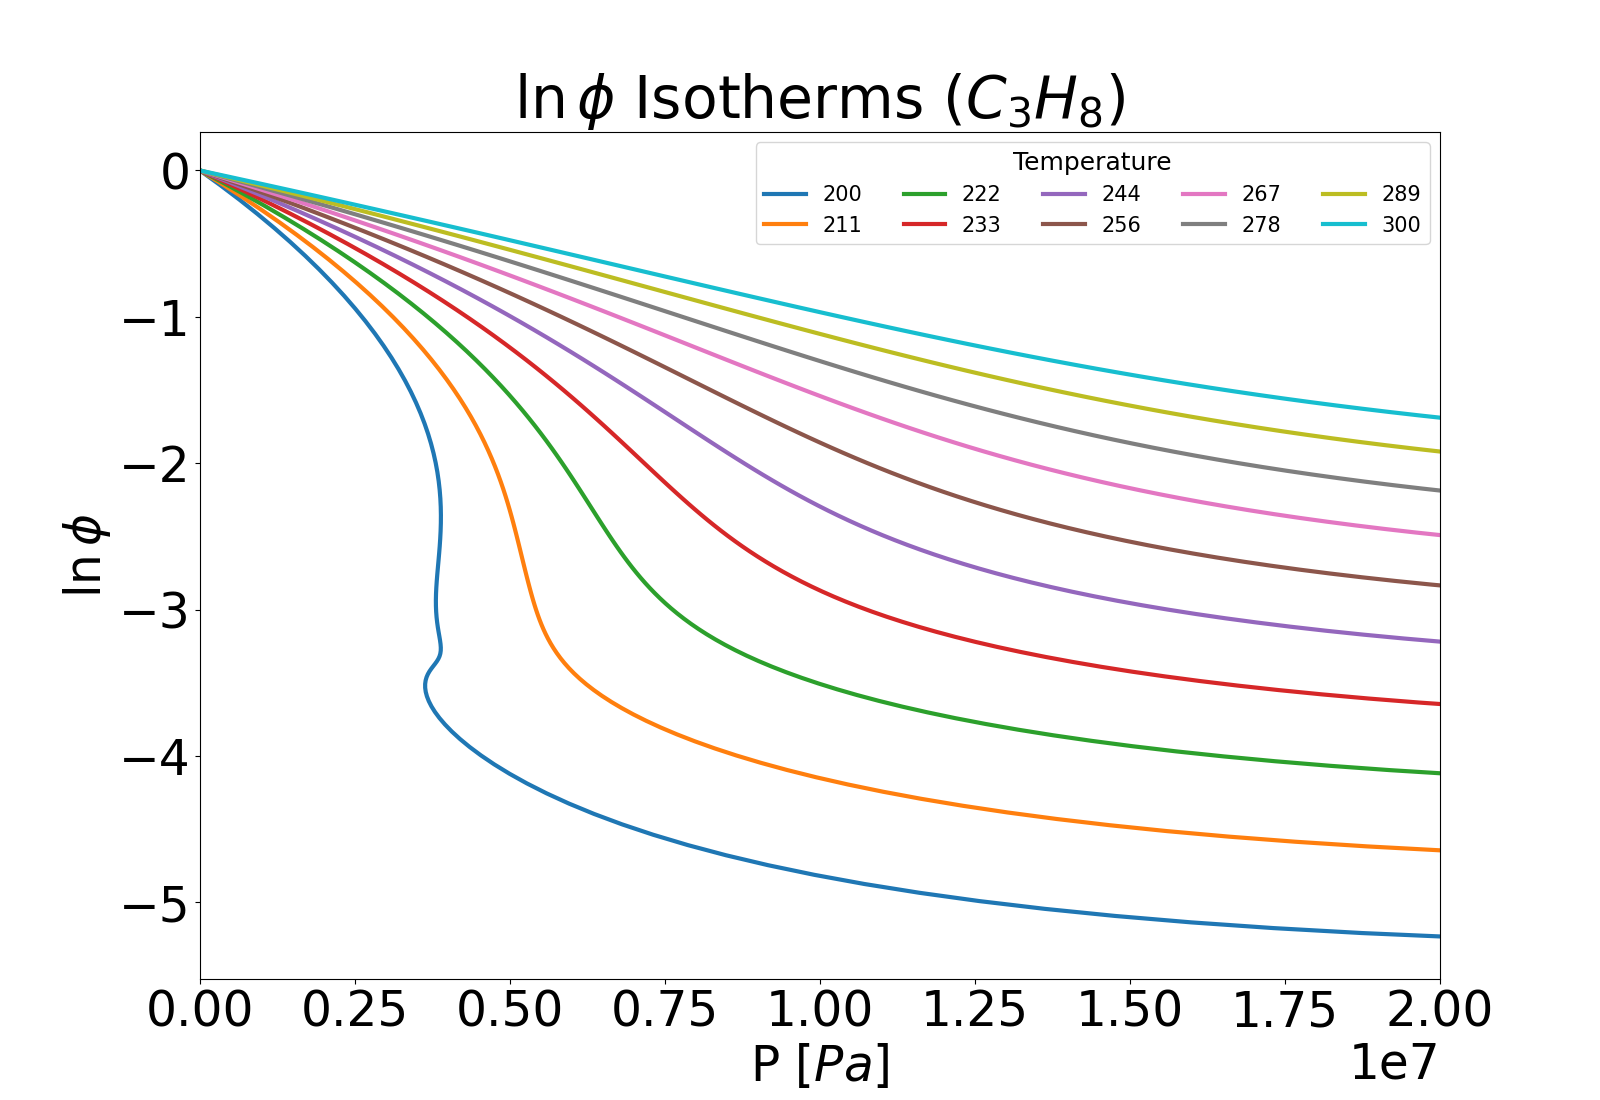
\includegraphics[width=17cm]{lnfug.png}

\end{multicols}

\subsection*{Equilibrium procedures}
All the equilibrium related calculations are done by functions that receive a
fluid and another relevant variable (like pressure and temperature for a PT
Flash) and return a liquid and vapor \texttt{Fluid} objects.

\begin{multicols}{2}
    

\begin{minted}{python}
flash_pt = pff.equilibrium.flash_pt

composition = {'propane': 0.01, 'butane': 0.5, 'isobutane': 0.15,
               'pentane': 0.2, 'hexane': 0.14}
temperature = 366.48
pressure = 1.039e6

fluid = pff.Fluid(
    model=pff.models.GERG2008(),
    composition=composition,
    temperature=temperature,
    density=1,
)

vapor, liquid, beta, it = flash_pt(fluid, pressure, temperature)

>>> vapor
>>> Fluid(model=GERG2008, temperature=366.48, pressure=1039000.0000, 
          density=0.4236, 
          composition={
          'propane': 0.02405919, 'butane': 0.59222959, 
          'isobutane': 0.22051554, 'pentane': 0.11992022, 'hexane': 0.04327129
          }
    )
\end{minted}

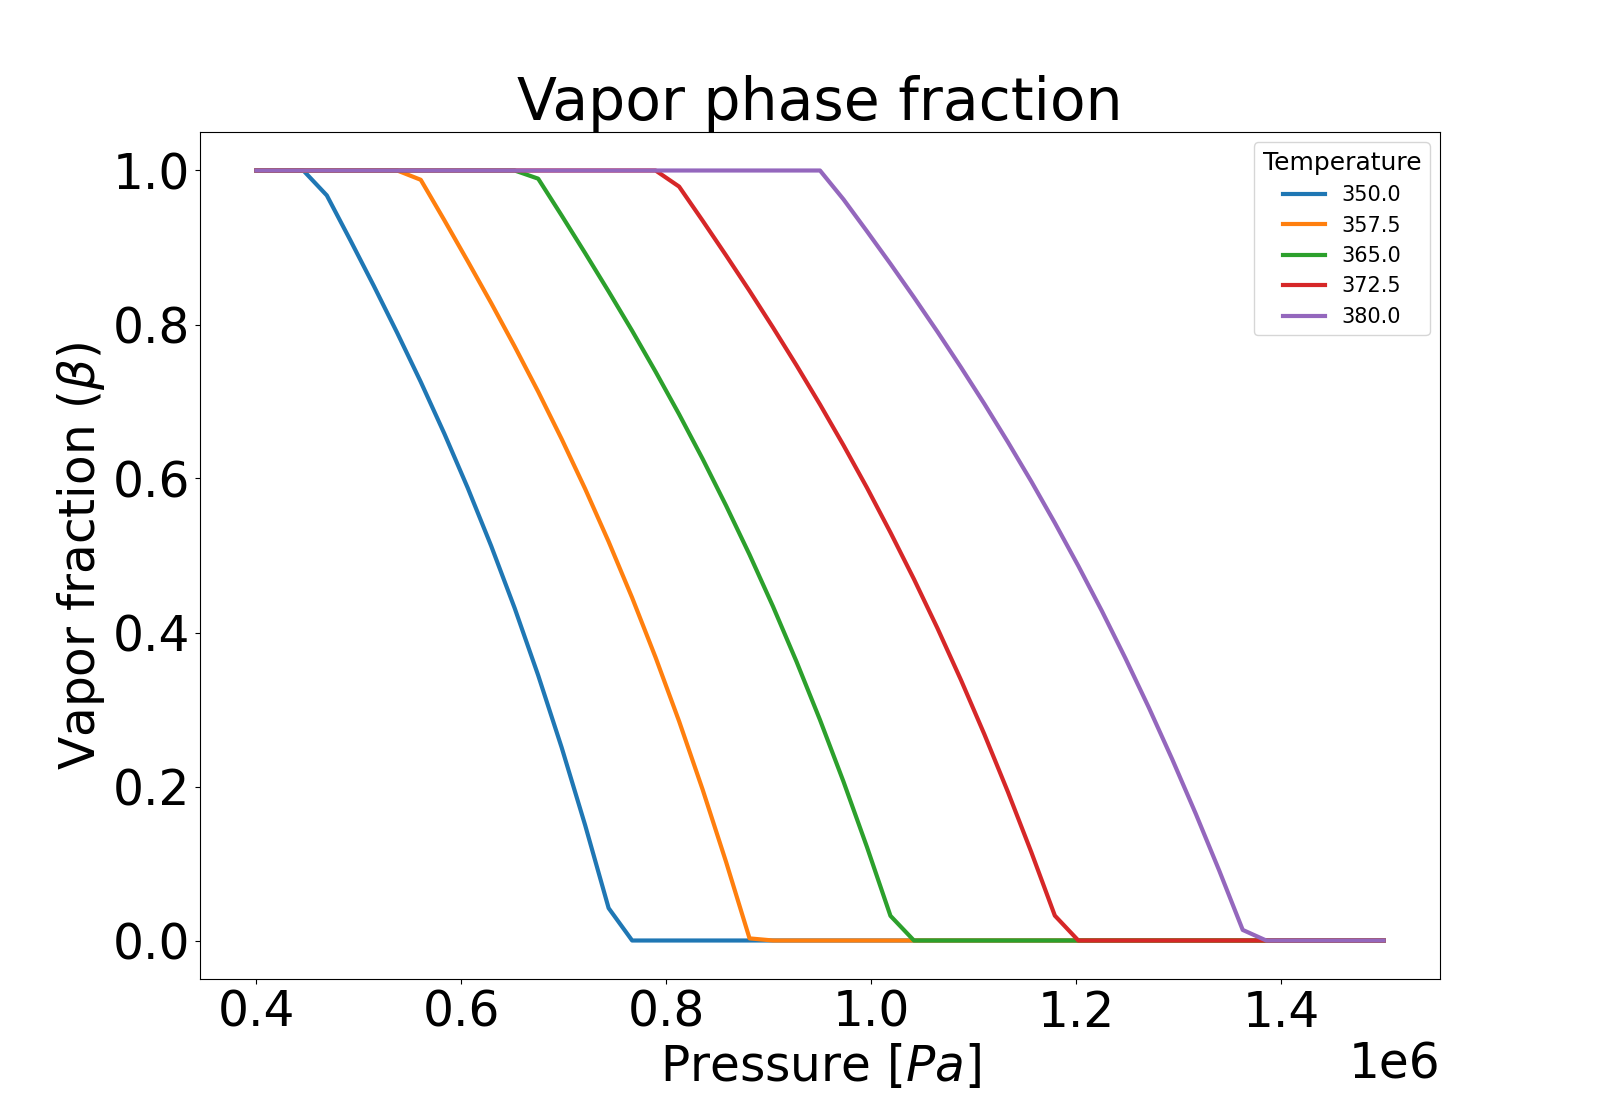
\includegraphics[width=17cm]{beta.png}
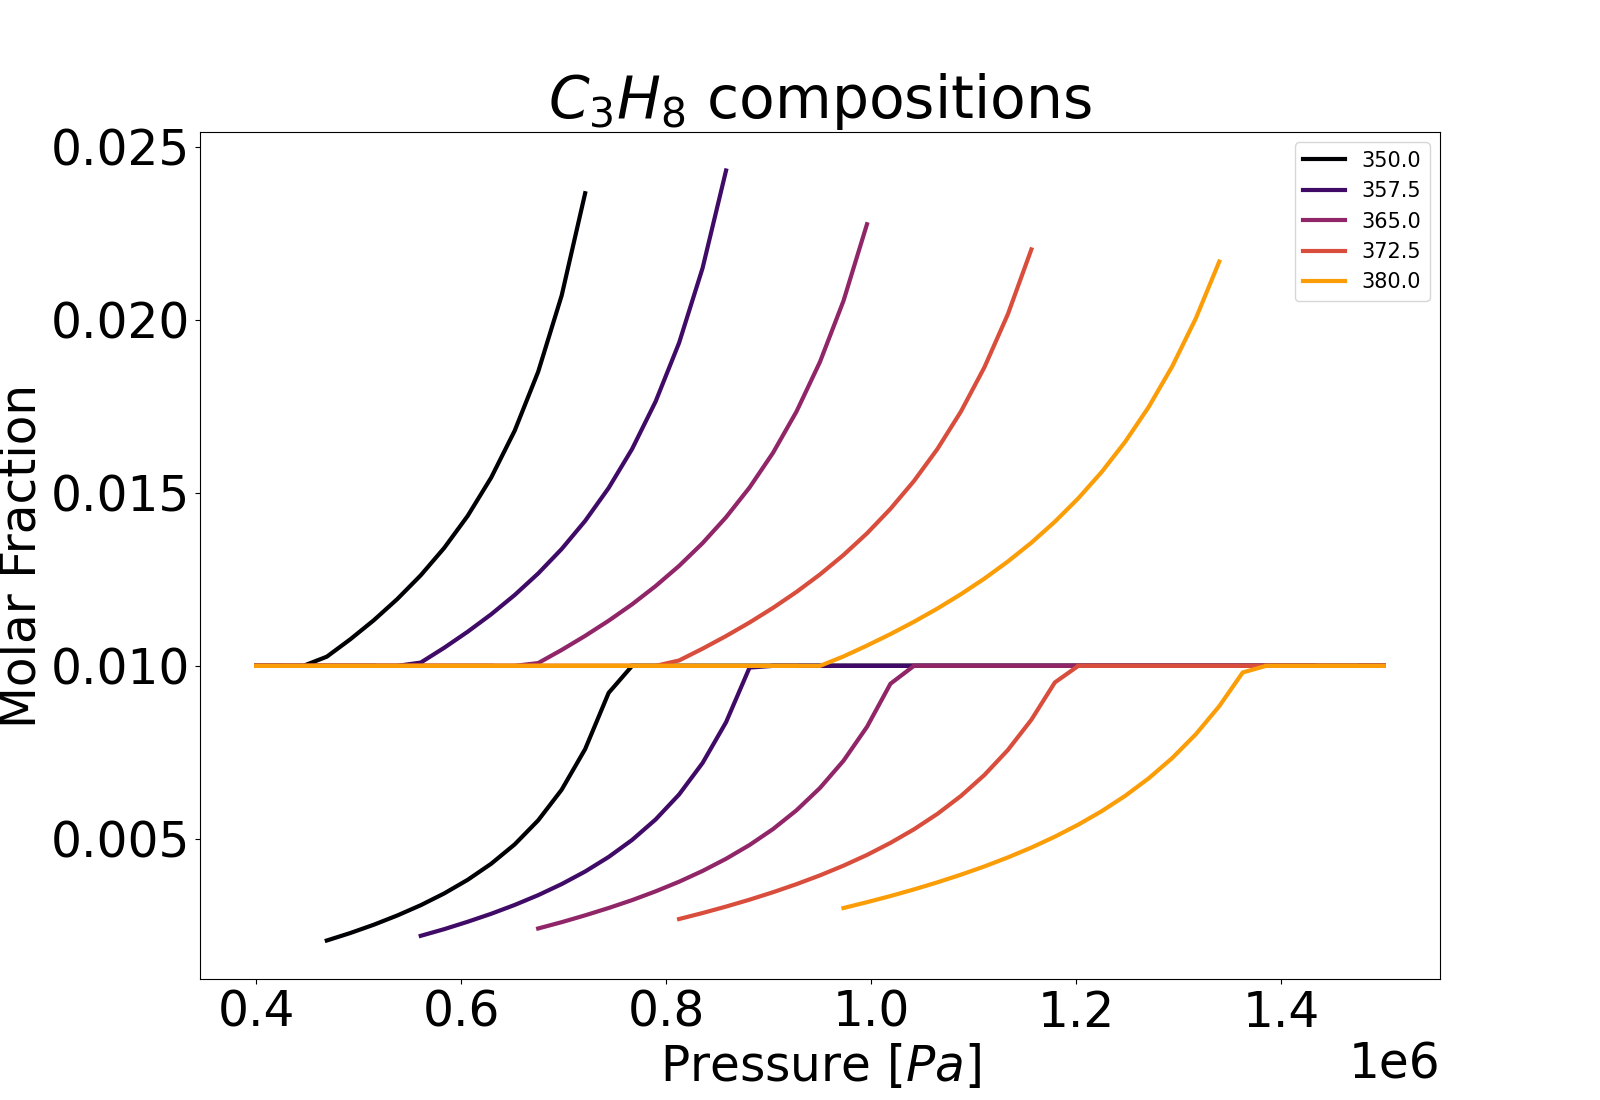
\includegraphics[width=17cm]{flashes.png}

\end{multicols}

\section*{Code Quality}
All the produced code is hosted online at
https://github.com/fedebenelli/pyforfluids. At each code commit a set of unit
tests is run that assure the correct work of the package, as well that
codestyle rules are respected. Forcing that at least 90\% of the code is
tested. All the procedures are documented and hosted at
\texttt{pyforfluids.readthedocs.io}

\nocite{*} % Print all references regardless of whether they were cited in the poster or not
%\bibliographystyle{plain}

\printbibliography
%\bibliography{./sample.bib} % Use the example bibliography file sample.bib

\end{multicols}
\end{document}
